\documentclass[12pt]{article}
\usepackage[utf8]{inputenc}
\usepackage[english]{babel}
\usepackage[letterpaper, portrait, margin=1in]{geometry}
\usepackage{amsmath}
\numberwithin{equation}{section}
\usepackage{amssymb}
\usepackage{graphicx}
\usepackage{parskip}
\usepackage{xcolor}
\usepackage{physics}
\usepackage{empheq}
\usepackage{cancel}
\usepackage{hyperref}
\hypersetup{colorlinks = true, urlcolor = blue, linkcolor = red, citecolor = red}
\usepackage{enumerate}
\usepackage{tikz}
\usepackage{float}
\usepackage{tcolorbox}
\usepackage{booktabs}
\usepackage[bottom]{footmisc}

% Default fixed font does not support bold face
\DeclareFixedFont{\ttb}{T1}{txtt}{bx}{n}{12} % for bold
\DeclareFixedFont{\ttm}{T1}{txtt}{m}{n}{12}  % for normal

% Custom colors
\usepackage{color}
\definecolor{deepblue}{rgb}{0,0,0.5}
\definecolor{deepred}{rgb}{0.6,0,0}
\definecolor{deepgreen}{rgb}{0,0.5,0}

\usepackage{listings}

% Python style for highlighting
\newcommand\pythonstyle{\lstset{
language=Python,
basicstyle=\ttm,
morekeywords={self},              % Add keywords here
commentstyle=\color{gray},
keywordstyle=\ttb\color{deepblue},
emph={MyClass,__init__},          % Custom highlighting
emphstyle=\ttb\color{deepred},    % Custom highlighting style
stringstyle=\color{deepgreen},                        % Any extra options here
showstringspaces=false
}}


% Python environment
\lstnewenvironment{python}[1][]
{
\pythonstyle
\lstset{#1}
}
{}

% Python for external files
\newcommand\pythonexternal[2][]{{
\pythonstyle
\lstinputlisting[#1]{#2}}}

% Python for inline
\newcommand\pythoninline[1]{{\pythonstyle\lstinline!#1!}}

\usepackage{xcolor}
\usepackage{fancyhdr}
\pagestyle{fancy}
\fancyhf{}
\fancyfoot[C]{\color{lightgray} Python Lecture V Notes}
\fancyfoot[L]{\color{lightgray} \today}
\fancyfoot[R]{Page \thepage}
\renewcommand{\headrulewidth}{0pt}
\renewcommand{\footrulewidth}{0pt}
\begin{document}

\section{Review}

\textbf{Last time:}
\begin{itemize}
    \item Python miscellany
    \item Questions?
    \item Today: Numpy
\end{itemize}

\section{Numpy Basics}
\begin{itemize}
    \item NumPy (Numerical Python) is a python package for working with numerical data
    \item numpy is the standard for data analysis and is used in MANY other scientific packages---it's very important that you're familiar with Python
    \item Numpy should come with your Anaconda distribution.
    \item If you don't have numpy, install on the command line: \verb|pip install numpy|
    \item To import numpy
    \begin{python}
    import numpy as np
    \end{python}
\end{itemize}

\section{ndarray}
\begin{itemize}
    \item An n-dimensional array of items of the SAME type.
    \item ndarrays are faster and take up less memory than Python lists
    \item It is MUCH easier to perform calculations using ndarrays (we'll discuss this more!)
    \item numpy arrays have a shape given by a tuple. \verb|(rows, cols)| for 2d arrays.
\end{itemize}

\textbf{ndarray example}:
\begin{python}
import numpy as np
a = array([[ 0,  1,  2,  3,  4],
           [ 5,  6,  7,  8,  9],
           [10, 11, 12, 13, 14]])

>>> a.shape
(3,5)
>>> a.ndim
2
>>> a.dtype.name
'int64'
>>> a.size
15
\end{python}

\textbf{Creating arrays:}
\begin{itemize}
    \item We can create arrays from an existing list \pythoninline{a = np.array([[2,3,4], [5,6,7])}
    \item Ones and zeros:
    \begin{python}
    >>> np.zeros((3, 4))
    array([[0., 0., 0., 0.],
           [0., 0., 0., 0.],
           [0., 0., 0., 0.]])
           
    >>> # dtype can also be specified
    >>> # This is a 3d array! (we'll talk about axes in a bit!)
    >>> np.ones((2,3,4), dtype=np.int16) 
    array([[[1, 1, 1, 1],
            [1, 1, 1, 1],
            [1, 1, 1, 1]],
    
           [[1, 1, 1, 1],
            [1, 1, 1, 1],
            [1, 1, 1, 1]]], dtype=int16)
    \end{python}
    \item Create a seqeunce:
    \begin{python}
    # evenly spaced range arange([start], stop, [step])
    >>> np.arange( 10, 30, 5 )
    array([10, 15, 20, 25])
    
    # specify a number of elements across a range 
    # linspace(start, stop, num)
    >>> np.linspace(0, 1, 5)
    array([0.  , 0.25, 0.5 , 0.75, 1.  ])
    \end{python}
\end{itemize}

\textbf{numpy axes}:
    \begin{itemize}
        \item Often a very confusing topic!
        \begin{figure}[H]
	    \centering
	    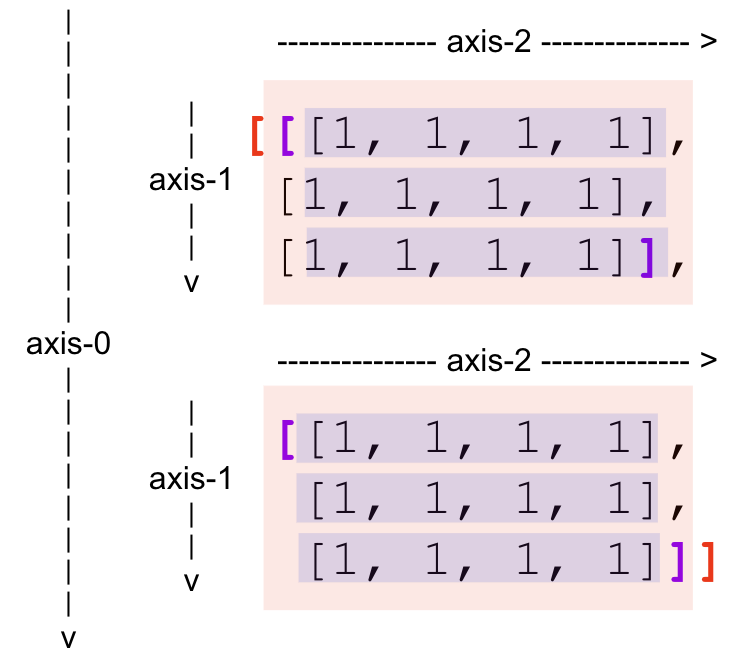
\includegraphics[width=6.5cm] {axes}
        \end{figure}
        
        \item Each dimension corresponds to an axis
        \item The axis convention is \textbf{OUT TO IN}. For example: the 3d array in the figure above has 3 degrees of freedom:
        \begin{itemize}
            \item \textbf{axis-0}: which one of the \textbf{two} 2d arrays? (\verb|a[0]| or \verb|a[1]|)
            \item \textbf{axis-1}: given one of the 2d arrays, which of the \textbf{three} 1d arrays (\verb|a[i,0]| or \verb|a[i,1]| or \verb|a[i,2]|)
            \item \textbf{axis-2:} given one of the 1d arrays, which of the \textbf{four} elements? (\verb|a[i,j,0]| or \verb|a[i,j,1]| or \verb|a[i,j,2]| or \verb|a[i,j,3]|)
        \end{itemize}
        \item For 2d array: \verb|(row, col)|. For 3d array: \verb|(matrix, row, col)|.
        \item This is why the array has shape \verb|(2,3,4)|
    \end{itemize}
    
\textbf{Practice with array indexing: }
\begin{python}
>>> a = np.arange(24).reshape((2,3,4))
>>> a
array([[[ 0,  1,  2,  3],
        [ 4,  5,  6,  7],
        [ 8,  9, 10, 11]],

       [[12, 13, 14, 15],
        [16, 17, 18, 19],
        [20, 21, 22, 23]]])

# What is a[1]?
# What is a[1,2]?
# What is a[1,2,3]

# Notice: array slicing still works!
# Notice: a[1] = a[1,:,:] = a[1:...]

# REMEMBER: read left to right, out to in
# What is a[0,0,2:]?
# What is a[0,:,2:]?
# What is a[:,:2,2:]?
\end{python}

\textbf{Manipulating arrays} (you can read up on your own):
\begin{itemize}
    \item \verb|np.reshape|
    \item \verb|np.concatenate|
    \item \verb|np.stack|, \verb|np.vstack, np.hstack, np.vsplit, np.hsplit|, \verb|np.column_stack|
\end{itemize}

\section{Vectorized Operations}
\begin{itemize}
    \item Often times, we want to perform element-wise operations on an array. (For example, we want to multiply all elements by some factor). This is called a VECTORIZED operation.
    \item How would we do this with lists?
    \begin{python}
    a = [[1,2,3], [4,5,6]]
    # what happens when we do 3*a? (it ends badly)
    
    for row in range(len(a)):
        for col in range(len(a[0])):
            a[i][j] = 3 * a[i][j]
    \end{python}
    This is SLOW and ANNOYING to write. It's also hard to quickly understand what the code is doing!
    \item In numpy, mathematical operations are vectorized!
    \begin{python}
    a = np.array(a)
    a = 3 * a
    
    >>> a
    array([[ 3,  6,  9],
           [12, 15, 18]])
    \end{python}
    Numpy's vectorized operations are implemented in C, so they are FAST! With numpy, it is easier to perform element-wise operations and it's easier to read!
\end{itemize}
\begin{figure}[H]
	\centering
	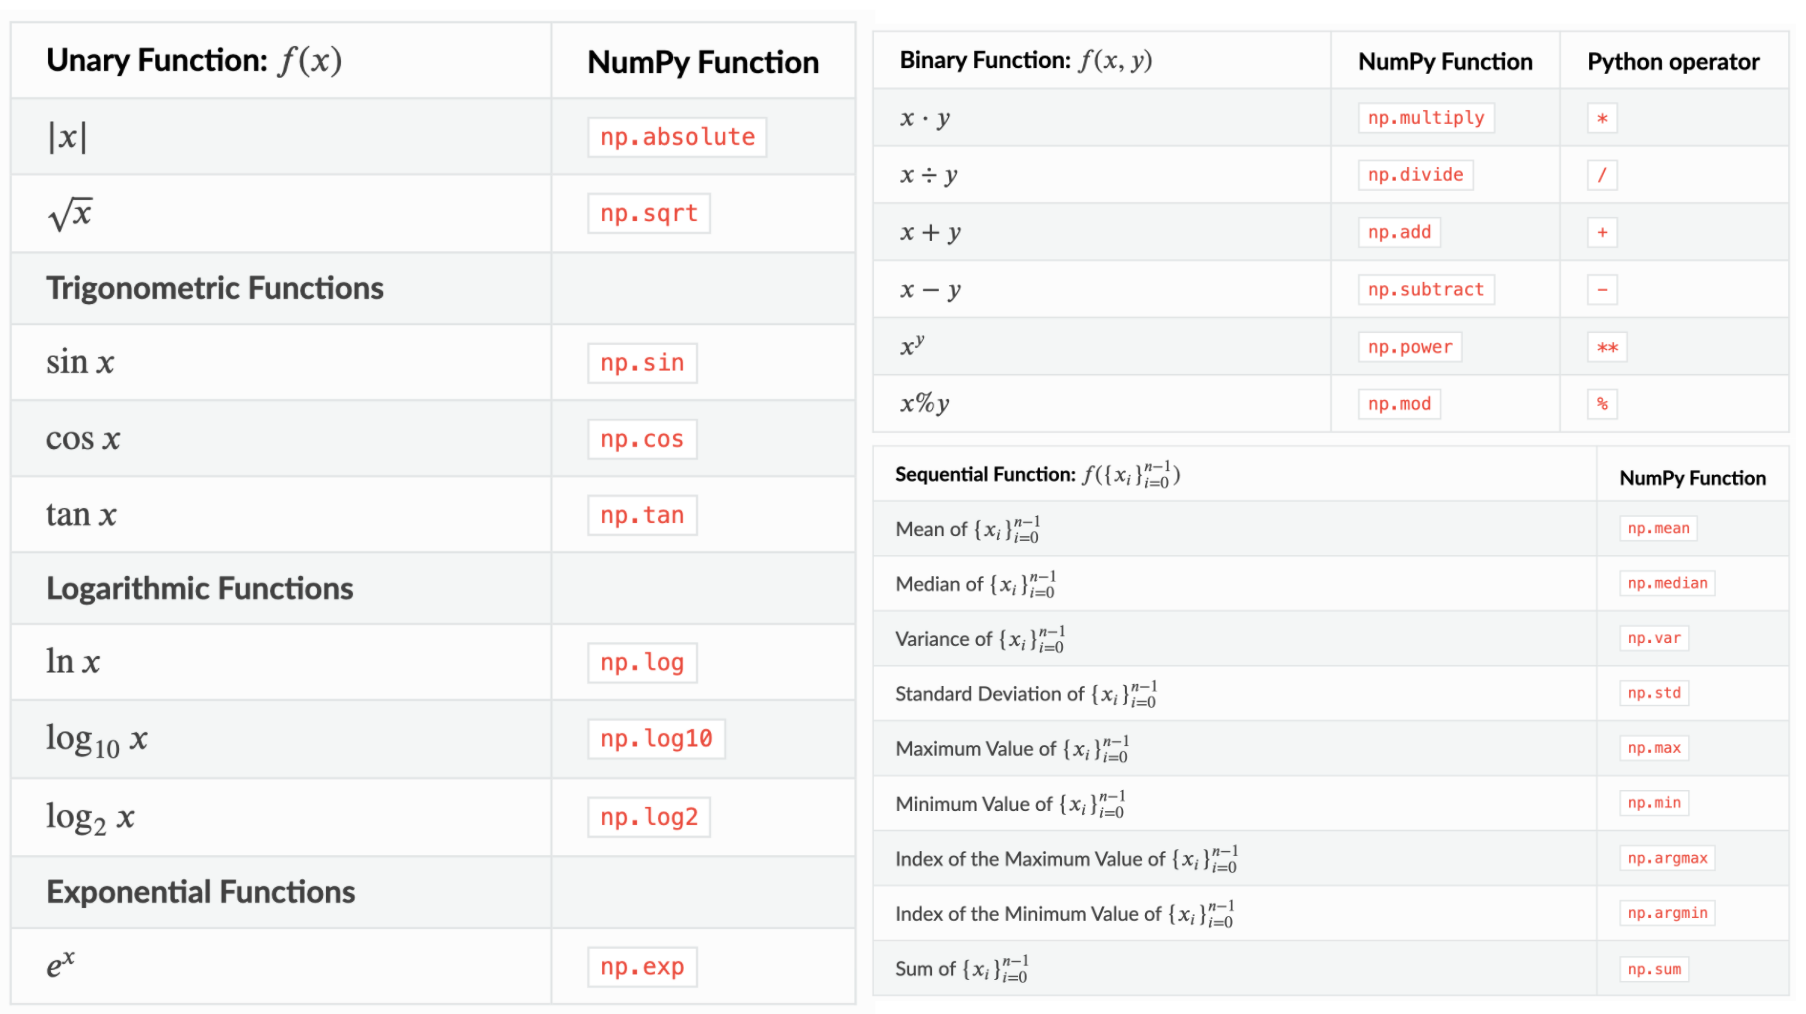
\includegraphics[width=16.5cm] {vector}
\end{figure}

\textbf{Example:}
\begin{python}
>>> x = np.arange(5)
>>> x
array([0, 1, 2, 3, 4])

>>> y = 5*x + 1
>>> y
array([ 1,  6, 11, 16, 21])

# operations between two numpy arrays are STILL element-wise
>>> x + y
array([ 1,  7, 13, 19, 25])
>>> x * y
array([ 0,  6, 22, 48, 84])

>>> np.max(y)
21
>>> np.mean(y)
11.0
\end{python}
\textbf{We can specify the axis of an operation:}
\begin{python}
>>> a = np.arange(24).reshape((2,3,4))
>>> a
array([[[ 0,  1,  2,  3],
        [ 4,  5,  6,  7],
        [ 8,  9, 10, 11]],

       [[12, 13, 14, 15],
        [16, 17, 18, 19],
        [20, 21, 22, 23]]])

>>> # sum ALONG the 0 axis
>>> np.sum(a, axis=0)
array([[12, 14, 16, 18],
       [20, 22, 24, 26],
       [28, 30, 32, 34]])
\end{python}

\textbf{Numpy also supports vectorized logical operations: }
\begin{python}
>>> a = np.arange(24).reshape((2,3,4))
>>> a%2 == 0
array([[[ True, False,  True, False],
        [ True, False,  True, False],
        [ True, False,  True, False]],

       [[ True, False,  True, False],
        [ True, False,  True, False],
        [ True, False,  True, False]]])
>>> np.where(a%2 == 0)
(array([0, 0, 0, 0, 0, 0, 1, 1, 1, 1, 1, 1]), 
 array([0, 0, 1, 1, 2, 2, 0, 0, 1, 1, 2, 2]), 
 array([0, 2, 0, 2, 0, 2, 0, 2, 0, 2, 0, 2]))
>>> a[np.where(a%2 == 0)]
array([ 0,  2,  4,  6,  8, 10, 12, 14, 16, 18, 20, 22])
\end{python}

\section{Additional}
Numpy has much more functionality that we won't have the chance to cover (to name a few):
\begin{itemize}
    \item Random
    \item Linear algebra (linalg)
    \item Fast Fourier Transfor (fft)
\end{itemize}

\textbf{Read more about Numpy:}
\begin{itemize}
    \item \url{https://numpy.org/doc/stable/contents.html}
    \item \url{https://www.pythonlikeyoumeanit.com/module_3.html}
\end{itemize}   

\section{Next Time}
\begin{itemize}
    \item Pandas
    \item Plotting in python with Matplotlib
\end{itemize}

\appendix
\section{(Optional) Array Broadcasting}
When two arrays have the same shape, we can easily understand what an element-wise operation does---it applies some operation between corresponding elements of the arrays!

For example (both arrays have \verb|shape=(2,3)|),
\begin{equation*}
    \begin{pmatrix}
        1 & 2 & 3\\
        4 & 5 & 6\\
    \end{pmatrix}
    +
    \begin{pmatrix}
        1 & 1 & 1\\
        2 & 2 & 2\\
    \end{pmatrix}
    \xrightarrow{element-wise }
    \begin{pmatrix}
        2 & 3 & 4\\
        6 & 7 & 8\\
    \end{pmatrix}
\end{equation*}

However, we can use BROADCASTING to perform operations on arrays of UNEQUAL shapes IF they are broadcastable. For example, adding a \verb|(3,2)| array to a \verb|(2,)| array:

\begin{equation*}
    \begin{pmatrix}
        1 & 2\\
        3 & 4\\
        5 & 6\\
    \end{pmatrix}
    +
    \begin{pmatrix}
        1 & 2\\
    \end{pmatrix}
    \xrightarrow{broadcast }
    \begin{pmatrix}
        1 & 2\\
        3 & 4\\
        5 & 6\\
    \end{pmatrix}
    +
    \begin{pmatrix}
        1 & 2\\
        1 & 2\\
        1 & 2\\
    \end{pmatrix}
    \xrightarrow{element-wise }
	\begin{pmatrix}
		2 & 4\\
		4 & 6\\
		6 & 8\\
	\end{pmatrix}
\end{equation*}

\textbf{Broadcasting steps} (using example above):
\begin{enumerate}
    \item Determine the shape of both arrays: \verb|(3,2)| and \verb|(2,)|
    \item If the shapes are not the same size, \textbf{prepend} the smaller shape with 1's until both arrays have the same number of dimensions. In this case, the first shape has dimension 2, so we must extend the second shape: \verb|(2,)| $\rightarrow$ \verb|(1,2)|
    \item Align the array dimensions:
    \begin{align*}
        &\text{(3, 2)}\\
        &\text{(1, 2)}
    \end{align*}
    The respective dimensions must be (a) equal or (b) one of them is 1. \textbf{Otherwise, the arrays can not be broadcast.} In this case, axis-0 (3 and 1) are not equal but contains one 1, and axis-1 (2 and 2) are equal.
    \item If the respective dimensions are equal, the operation is applied element wise. If the respective dimensions are not equal, but one dimension is 1, then the dimension 1 is broadcast.
\end{enumerate}

   This is fully generalized. However, broadcasting can get nasty with high dimensions. As always, if you're getting lost in the complexity of your data, you should probably reconsider it's format. 

\end{document}
